\documentclass{beamer}
\mode<presentation> 
{
	\usetheme[alternativetitlepage]{Torino}
	\usecolortheme{chameleon}
	\setbeamercovered{transparent}	
}
\usepackage{ucs}
\usepackage[utf8x]{inputenc}
\usepackage[czech]{babel}
\usepackage{palatino}
\usepackage{graphicx}
\usepackage{epstopdf}
\usepackage{color}
\usepackage[export]{adjustbox}
\usepackage{multicol}
\usepackage{hyperref}
\usepackage{subcaption}
\usepackage{caption}
\captionsetup{labelformat=empty,labelsep=none}


\definecolor{olive}{RGB}{51, 149, 48}
\definecolor{red}{RGB}{195, 2, 36}

\definecolor{gred}{RGB}{196, 66, 48}
\definecolor{glime}{RGB}{168, 189, 4}
\definecolor{ggreen}{RGB}{57,181,74}

\title{\textbf{Aktuální vývoj WebGL}}
\author{
	\large{Pavel Macenauer} \\ 
	\tiny{xmacen02@stud.fit.vutbr.cz} \\ 
	\large{Jan Bureš} \\ 
	\tiny{xbures19@stud.fit.vutbr.cz}
}
\date{\tiny{\today}}
\institute[FIT VUTBR]
{
	\inst{}
	Fakulta Informačních Technologií \\
	Vysoké Učení Technické v Brně
}

\begin{document}

	\begin{frame}[t,plain]
	\titlepage
	\tableofcontents[currentsection]
	\vspace{-10mm}
	\center{ \includegraphics[height=9mm]{logo.eps} }
	\end{frame}

%% ------------- SNIMAC -------------

	\begin{frame}[t,fragile]
		\frametitle{Obsah}	
		
		\begin{itemize}
			\item WebGL
			\begin{itemize}
				\item Charakteristika
				\item Podpora v prohlížečích
				\item Historie
				\item Budoucnost
				\item Bezpečnost a IE11				
			\end{itemize}
			\item Alternativy kreslení na webu a srovnání s WebGL
			\item Přehled knihoven a herních enginů
			\item Emscripten
		\end{itemize}			
				
	\end{frame}
	
%% -----------------------------


	{
\usebackgroundtemplate{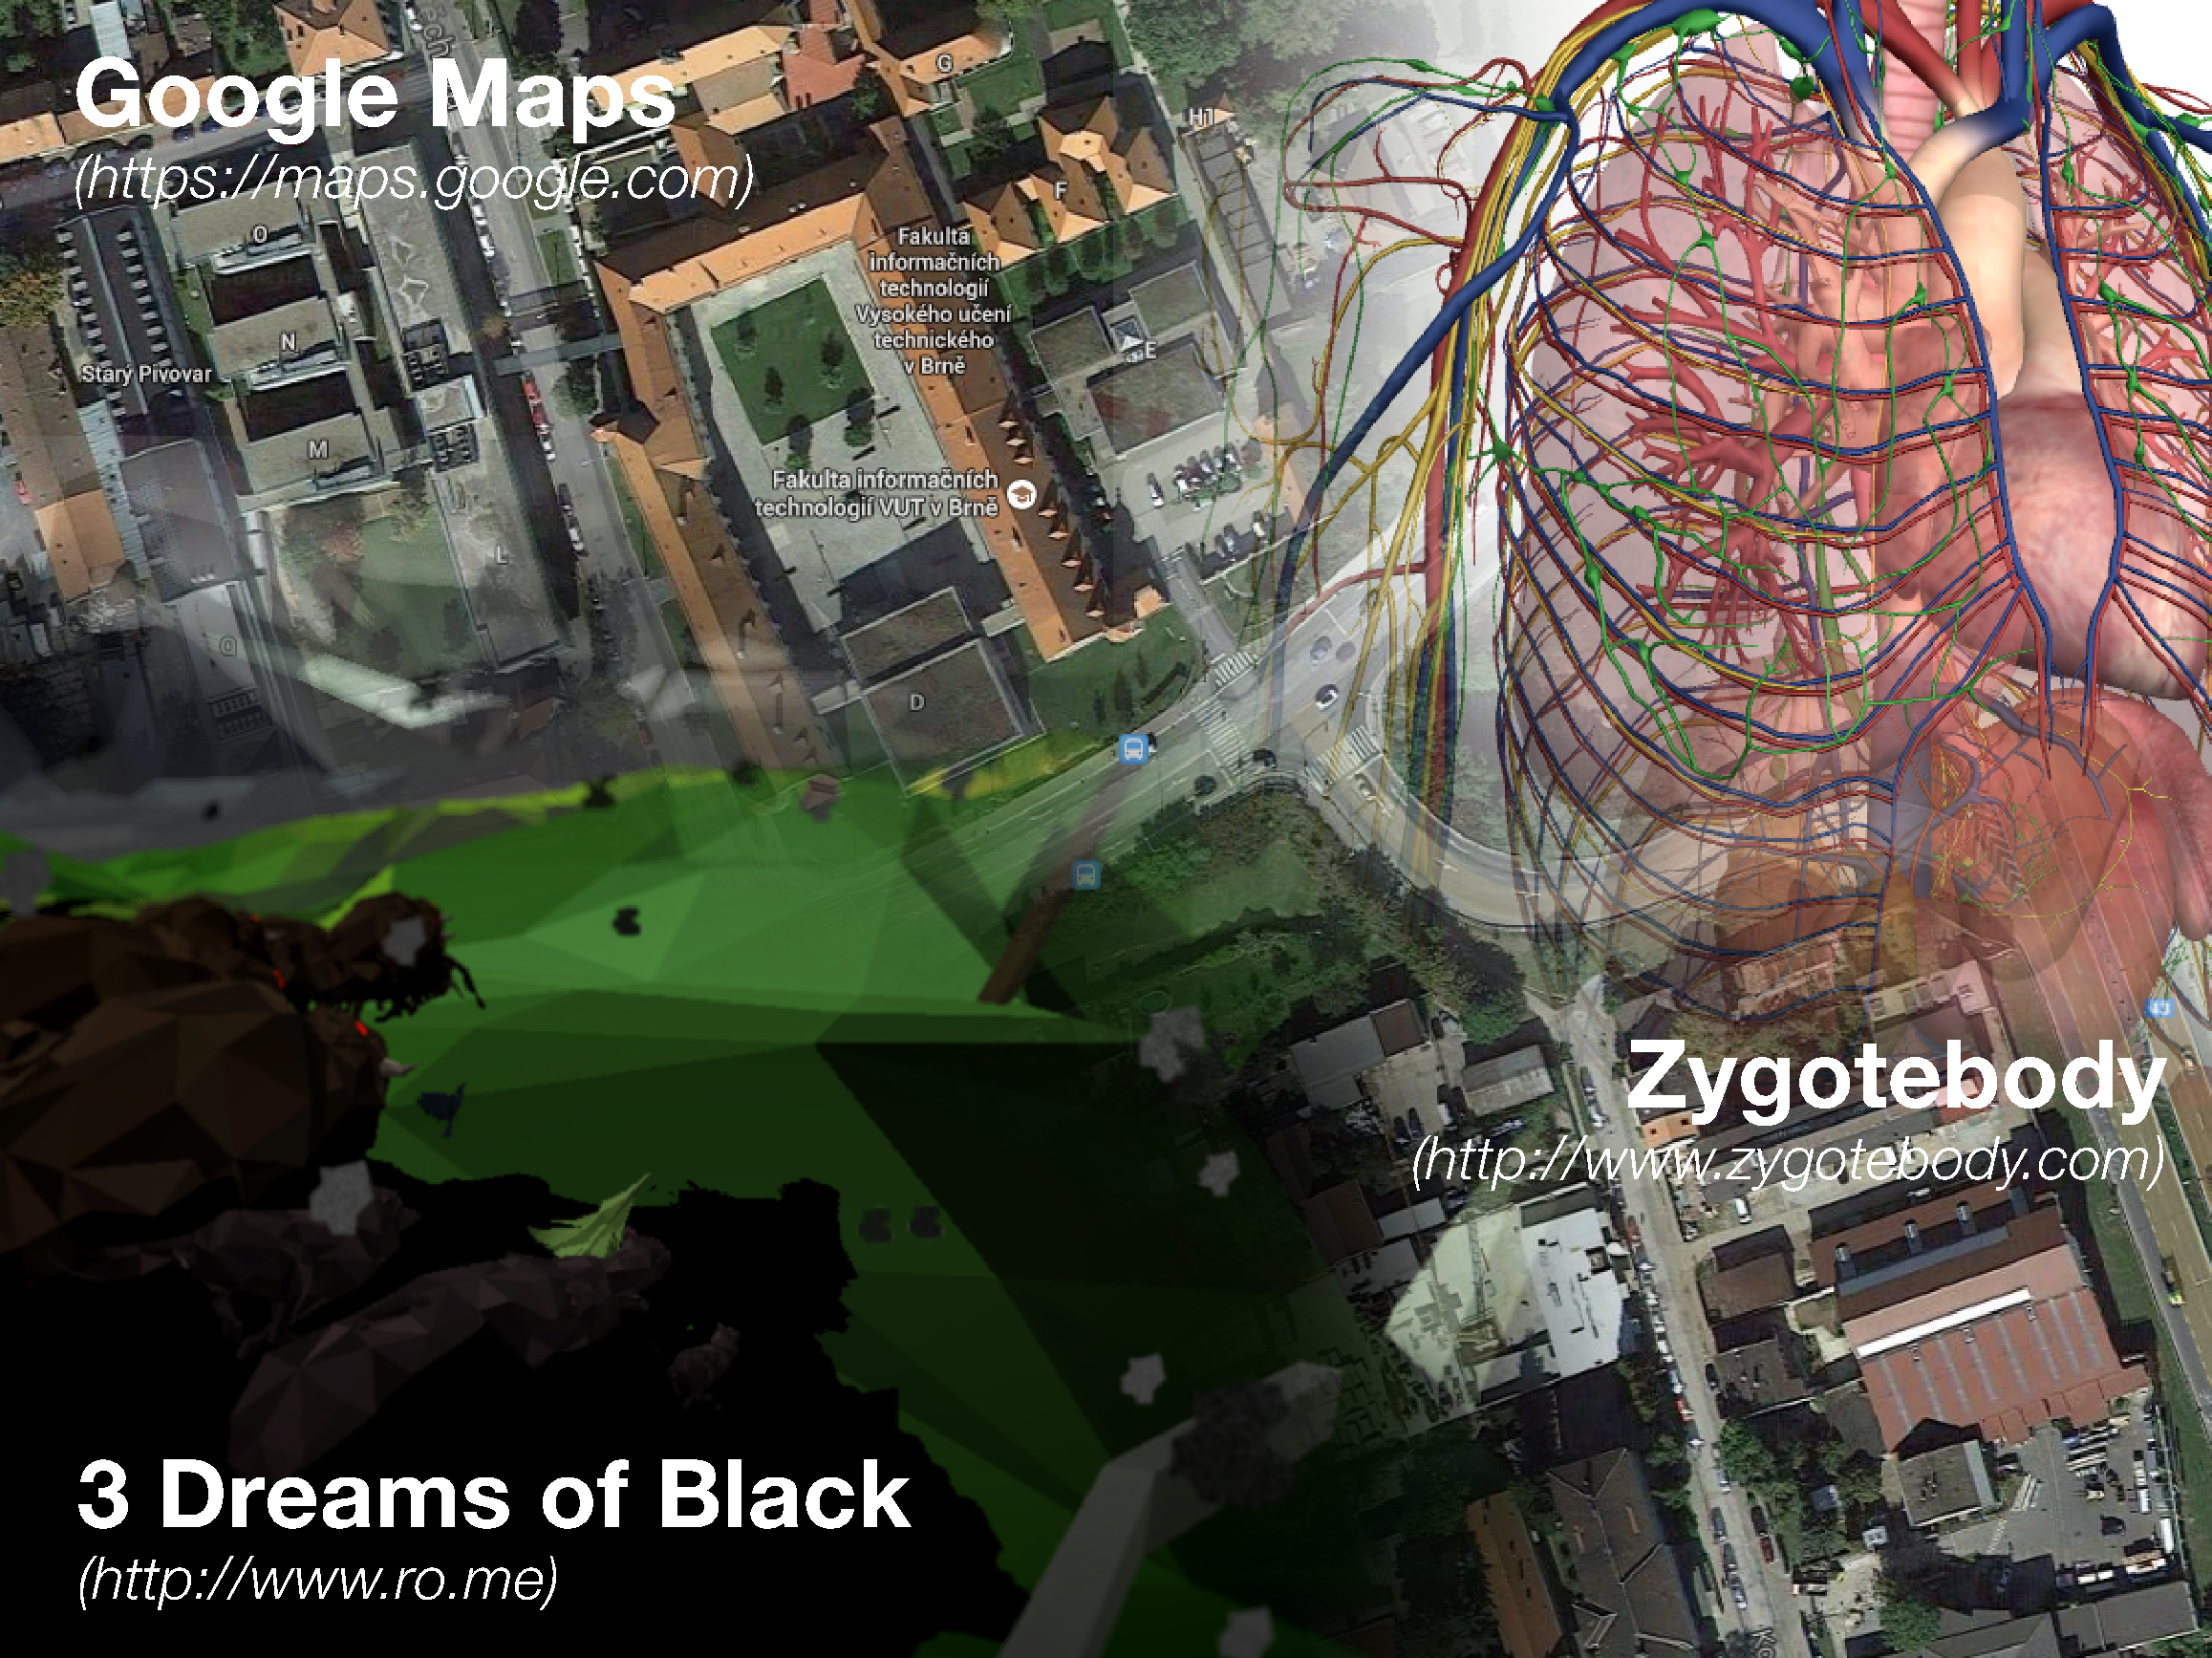
\includegraphics[width=\paperwidth]{img/example.pdf}}
\begin{frame}[plain]
\end{frame}
}
	
	%% -----------------------------
	
	\begin{frame}[t,fragile]
		\frametitle{WebGL - charakteristika}
		
		\begin{itemize}
			\item OpenGL na webových stránkách \\
				\footnotesize{nízkoúrovňové API pro práci s grafikou}
			\item \large{Vykreslováno v HTML5 elementu} \verb|<canvas>|
			\item \large{Khronos Group} \\
				\footnotesize{má na starosti specifikaci, členové jsou např. Google, Mozzila, Opera}
			\item \large{OpenGL ES 2.0 (WebGL 1.0.2) a OpenGL ES 3.0 (WebGL 2.0)}
			\item Dnes již podporováno ve všech běžně používaných prohlížečích
		\end{itemize}		
		
	\end{frame}



	
%% ------------------------------

	\begin{frame}[t,fragile]
		\frametitle{Podpora WebGL k listopadu 2014}
		
		\linebreak
		
		\centering
		\begin{figure}		
		\includegraphics[width=110mm]{img/webglsupport.png}
		\end{figure}
		\textcolor{ggreen}{plně podporováno} \\
		\textcolor{gred}{nepodporováno} \\
		\textcolor{glime}{částečně podporováno} *
		
	
		\flushleft
* \footnotesize{prohlížeče vyžadují konkrétní verze driverů, WebGL tak není podporováno na všech zařízeních}
			

	\end{frame}
	
		%% --------------------------

	\begin{frame}[t,fragile]
		\frametitle{Historie}					
		\begin{itemize}
	    	\item \textbf{2006} – Vladimir Vukićević - první prototyp
			\item \textbf{2007} – Mozzila Firefox a Opera podporují WebGL
			\item \textbf{2009} – Khronos group 
			\item \textbf{2011} – Oficiální specifikace WebGL 1.0
			\item \textbf{2013} – Specifikace WebGL 2.0
		\end{itemize}	
		
		\begin{figure}		
			\includegraphics[width=30mm]{img/vukicevic.jpg}
			\caption{Vladimir Vukićević na Mozzila konferenci v Kanadě}
		\end{figure}
		
	\end{frame}
	
	%% --------------------------
	
		\begin{frame}[t,fragile]
		\frametitle{Budoucnost}					
		\begin{itemize}
			\item OpenGL ES 3.1
			\begin{itemize}
				\item nepřímé vykreslovací příkazy
				\item výpočetní shadery
				\item vylepšené GLSL, texturovací funkcionalita, volitelná rozšíření, \dots
			\end{itemize}
			\item WebGL v mobilních prohlížečích
			\item Stále více uplatňováno v každodenních projektech
		\end{itemize}	
		
		\vspace{-3mm}				
		
		\begin{figure}
		\centering\begin{tabular}{ll}
			\includegraphics[height=28mm]{img/london.jpg} &		
			\includegraphics[height=28mm]{img/tokyo.jpg}
		\end{tabular}		
		\caption{3D obrázky z Google Maps - Londýn (vlevo), Tokyo (vpravo)}
		\end{figure}
									
	\end{frame}	
	
	%% --------------------------
	
	\begin{frame}[t,fragile]
		\frametitle{Podpora IE 11}					
		\begin{itemize}
	    	\item \textbf{2011} – Microsoft oznamuje, že nebude podporovat WebGL
			\item \textbf{2013} – Microsoft oznamuje podporu WebGL v IE11 \\
			\footnotesize{běh WebGL zabalen do DirectX runtimu}		
		\end{itemize}	
		
		\vspace{15mm}
		\centering
		\Huge{Co ho k tomu vedlo?}
		
		
		
	\end{frame}
	
%% --------------------------

	\begin{frame}[t,fragile]
		\frametitle{Bezpečnostní rizika}					
		\begin{itemize}
			\item Undefined behaviour - např. čtení pixelů mimo framebuffer
			\item Přístup do nealokované paměti
			\item Shadery - shadery musí být validovány
			\item DoS (scéna trvá moc dlouho vykreslit - počítač přestane reagovat)
			\item Čtení obrázků a videí z cizích zdrojů - musí být validováno přes CORS	
		\end{itemize}	

	\end{frame}
	
	

	
		%% --------------------------
	
		\begin{frame}[t,fragile]
		\frametitle{Alternativy ke kreslení na webu}					
		\begin{itemize}
		
		\item \textbf{DOM}
		\begin{itemize}
			\item objekty ukládáný přímo do DOMu (stromu) webové stránky jako objekty (rect, circle, \textcolor{red}{svg}, path, ...)
			\item velmi rychlé při malém počtu objektů, ale postupně zahlcuje DOM
			\item možnost vázat handlery na jednotlivé objekty
		\end{itemize}

		\item \textbf{Canvas}
		\begin{itemize}
			\item API elementu \verb|<canvas>|
			\item kreslení pomocí JS metod (např. arc(), fill(), lineTo(), \dots)
			\item problém vázat handlery na jednotlivé objekty, protože vše je uvnitř \verb|<canvas>|-u
		\end{itemize}				
				
		\end{itemize}	

	\end{frame}
	
		%% --------------------------
		
				{
\usebackgroundtemplate{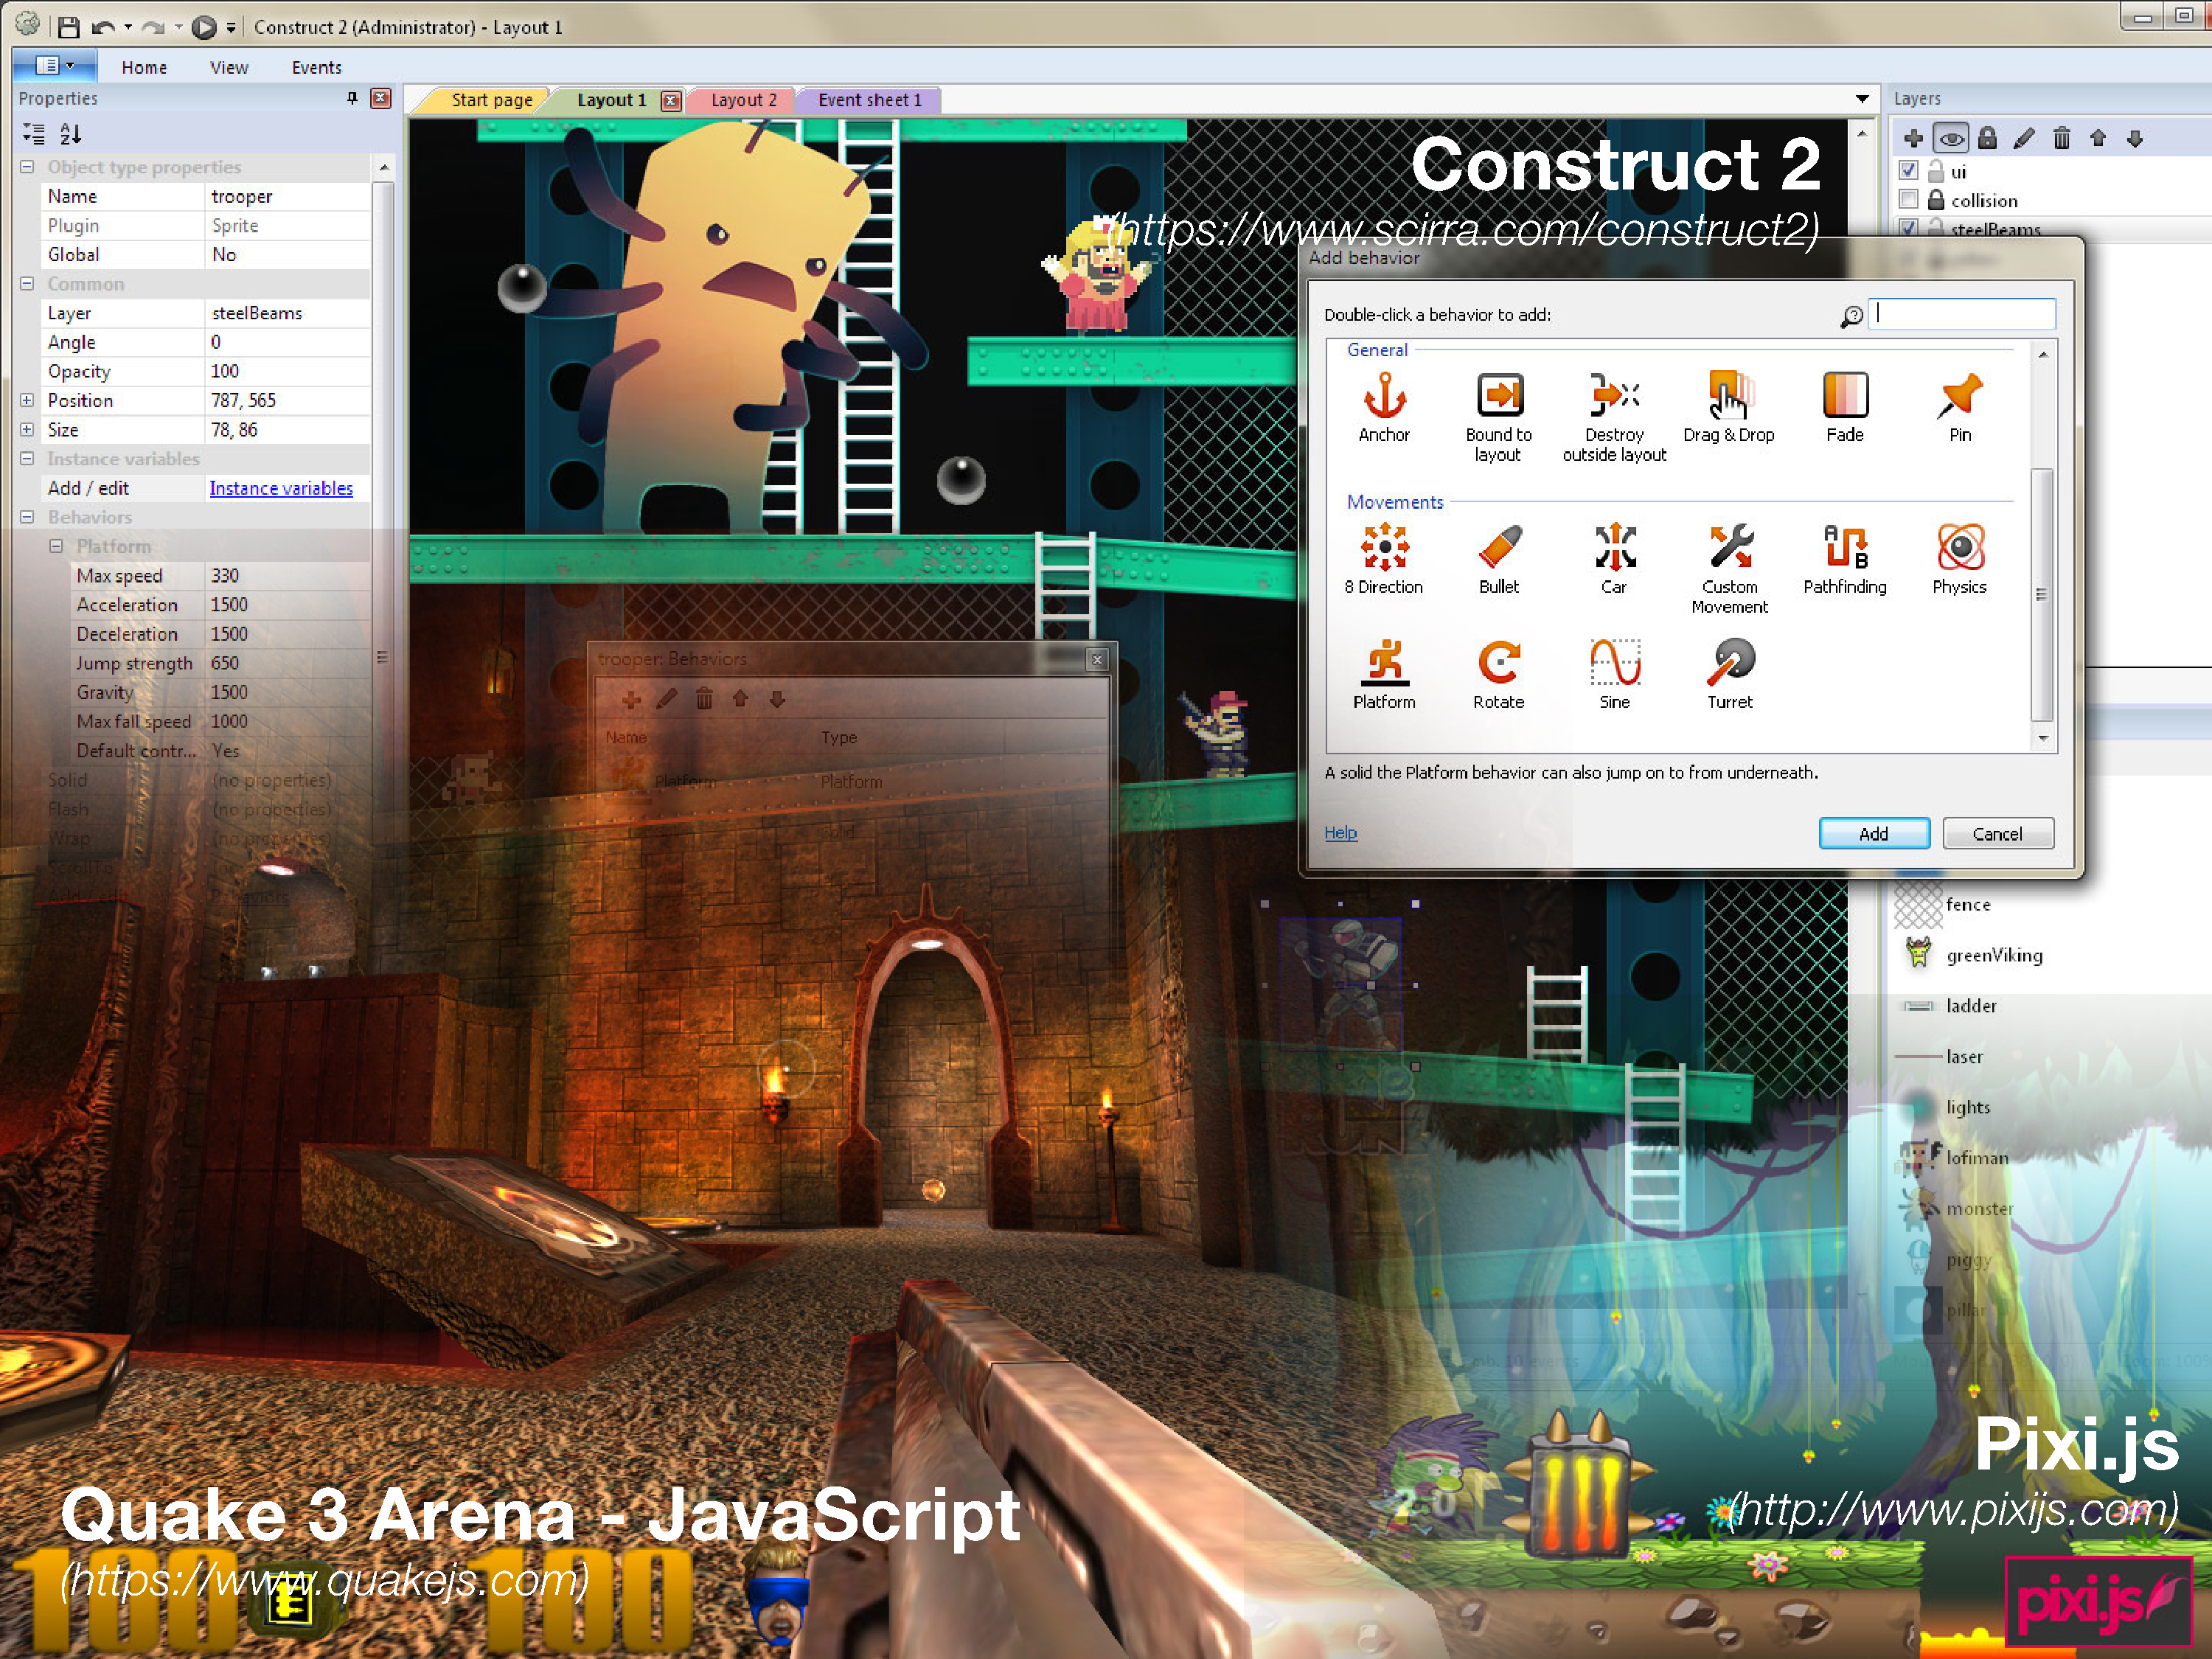
\includegraphics[width=\paperwidth]{img/example2.pdf}}
\begin{frame}[plain]
\end{frame}
}

		%% -----------------------------
	
		\begin{frame}[t,fragile]
		\frametitle{Přehled knihoven a herních enginů}					
		\begin{itemize}
		
		\item \textbf{Construct 2} (komerční pro komerční účely)
		\begin{itemize}
			\item 2D editor, jednoduché, časově nenáročné
			\item export pro HTML5, Chrome, Facebook, Windows Phone, přes wrappery jako Cocoon JS lze i pro Android nebo iOS
		\end{itemize}				
		\item \textbf{Three.js} (zdarma)
		\begin{itemize}
			\item 3D knihovna nad WebGL, ale využívá i Canvas/DOM fallback
			\item umí všechno možné			
		\end{itemize}				
		\item \textbf{pixi.js} (zdarma)
		\begin{itemize}
			\item 2D knihovna, ale má i Canvas fallback, Scene Graph
			\item WebGL postprocessing filtry, podpora více dotyků
			\item využívají i velké společnosti jako Google nebo McDonalds		
		\end{itemize}						
		\item \textbf{Isogenic} (komerční)
		\begin{itemize}
			\item client-server herní engine na masivně hrané multiplayer hry
			\item node.js, MongoDB, na kreslení využívá pouze DOM/Canvas a jednoduché metody		
		\end{itemize}				
		\end{itemize}	

	\end{frame}
	
	
	%% -----------------------------
	
		\begin{frame}[t,fragile]
		\frametitle{Další knihovny}					
		\begin{itemize}
				\item enchant.js \url{http://enchantjs.com/}
	\item PlayCanvas \url{https://playcanvas.com/}
	\item Phaser \url{http://phaser.io/}
	\item voxel.js \url{http://voxeljs.com/}
		\end{itemize}	

	\end{frame}
	
	%% -----------------------------
	
		\begin{frame}[t,fragile]
		\frametitle{Emscripten}					
		\begin{itemize}
			\item převod LLVM (výstup z C/C++ compileru) na JavaScript nebo asm.js
			\item asm.js - subjazyk javascriptu optimalizovaný pro cross-kompilaci
			\item podpora OpenGL, SDL
			\item DeadTrigger 2 (Unity 3D), Quake 3, Doom, Qt, Ruby, Python \dots
		\end{itemize}	
		\begin{figure}		
		\centering
		\includegraphics[height=40mm]{img/micro3b.png}
		\end{figure}

	\end{frame}
	
	%% -----------------------------
		
	\begin{frame}[t,fragile]
	
		\frametitle{Zajímavé zdroje}					
		\begin{itemize}
			\item \footnotesize{\url{http://kripken.github.io/mloc_emscripten_talk/#/}}
			\item \url{http://learningwebgl.com/}
			\item \url{http://www.chromeexperiments.com/webgl/}
			\item \url{https://www.shadertoy.com/}
		\end{itemize}			

	\end{frame}
	
	
\end{document} 
